% Implementation
\section{Implementation}

\kort{} wurde mit dem \brand{Sencha Touch 2}-Framework\footnote{\url{http://www.sencha.com/products/touch/}} erstellt. Zusätzlich wurden verschiedene Libraries und Community-Plugins eingesetzt, welche in der Tabelle \ref{table-kort-dependencies} beschrieben sind. 

\brand{Leaflet}\footnote{\url{http://leafletjs.com/}} wurde eingesetzt, um \brand{OpenStreetMap}-Daten auf der Karte anzuzeigen. Zusätzlich wurde das \emph{leaflet-osm}\footnote{\url{https://github.com/jfirebaugh/leaflet-osm}}-Plugin für Leaflet verwendet, um \brand{OpenStreetMap}-Objekte als \inlinecode{XML}-Code direkt auf der Karte darzustellen.

Für die Einbindung der Leaflet-Karte in Sencha Touch wurde das Plugin \brand{Ext.ux.LeafletMap} eingesetzt, welches ebenfalls während dieser Arbeit entwickelt wurde (siehe Abschnitt \ref{leaflet-sencha-komponente}).

Für die Internationalisierung des Frontends wurde das \brand{Ext.i18n.Bundle-touch}\footnote{\url{https://github.com/elmasse/Ext.i18n.Bundle-touch/tree/css-content}}-Plugin für Sencha Touch eingesetzt.

\begin{table}[H]
\centering
\begin{tabular}{|p{0.25\threecelltabwidth}|p{0.15\threecelltabwidth}|p{0.60\threecelltabwidth}|}
\hline 
\textbf{Library} & \textbf{Version} & \textbf{Verwendung} \\
\hline 
Sencha Touch 2 & 2.1.0 & Framework zur Erstellung von mobilen \glspl{WebApp} \\
\hline 
Sencha Cmd 2 & 3.0.0.250 & Build-Tool von Sencha \\
\hline 
Leaflet & 0.4.5 & Anzeige von \brand{OpenStreetMap}-Daten auf der Karte \\
\hline 
leaflet-osm & Git Revision 38665cc6c0 & Leaflet-Plugin zur Anzeige von \brand{OpenStreetMap}-Objekten auf der Karte \\
\hline 
Ext.ux.LeafletMap & 1.0.1 & Sencha Touch-Plugin zur Einbindung einer Leaflet-Karte in Sencha Touch \\
\hline 
Ext.i18n.Bundle-touch & Git Revision 
b4a0beaeb8 & Sencha Touch-Plugin zur Internationalisierung der Oberfläche \\
\hline 
\end{tabular}
\caption{Abhängigkeiten zu Libraries}
\label{table-kort-dependencies}
\end{table}

\subsection{Starten der App}
Beim Starten der App wird durch mehrere Entscheidungen festgelegt, welche Maske dem Benutzer angezeigt wird. In Abbildung \ref{image-kort-startup-activitydiagram} ist der Ablauf grob dargestellt.

Schlussendlich wird dem Benutzer eine der folgenden Masken angezeigt:

\begin{itemize}
\item \textbf{Hauptmaske}: Falls der Benutzer bereit ist, die App zu benutzen.
\item \textbf{Login Maske}: Falls der Benutzer noch nicht eingeloggt ist.
\item \textbf{Erste Schritte Maske}: Falls der Benutzer noch keinen Benutzernamen gewählt hat.
\item \textbf{Geolocation Fehler Maske}: Wenn keine Geolocation-Informationen verfügbar sind.
\end{itemize}

\begin{figure}[H]
	\centering
	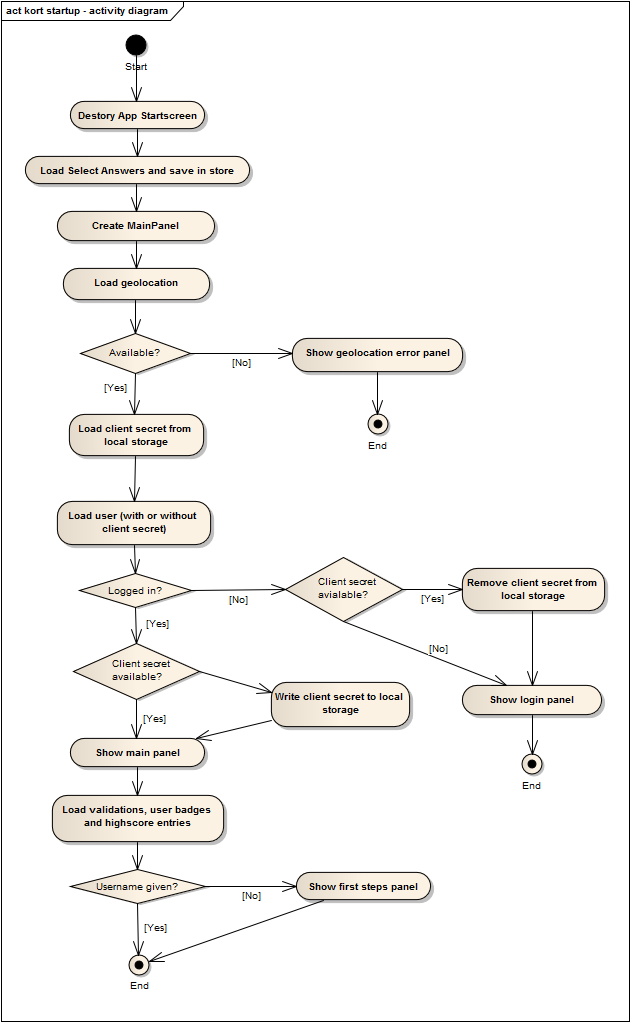
\includegraphics[scale=0.63]{images/uml/kort-startup-activitydiagram}
	\caption{Ablauf beim Starten der App}
	\label{image-kort-startup-activitydiagram}
\end{figure}

\subsection{Sencha Cmd}
\label{sencha-cmd}
Das Grundgerüst der App wurde komplett mit dem Sencha-eigenen Build-Tool \brand{Sencha Cmd}\footnote{\url{http://www.sencha.com/products/sencha-cmd}} generiert.
Dieses bietet verschiedene Build-Möglichkeiten an:

\begin{table}[H]
\centering
\begin{tabular}{|p{0.2\twocelltabwidth}|p{0.8\twocelltabwidth}|}
\hline
\textbf{Build} & \textbf{Beschreibung} \\
\hline
\inlinecode{testing} & Bei diesem Build werden die JavaScript-Quelldateien in einer Datei zusammengefasst. \\
\hline
\inlinecode{production} & Der Production-Build entspricht grundsätzlich dem Testing-Build. Zusätzlich werden aber die JavaScript-Quelldateien komprimiert. \\
\hline
\inlinecode{package/native} & Mit diesen Builds lassen sich native Apps für die verschiedenen mobilen Betriebssysteme generieren. \\
\hline
\end{tabular}
\caption{Build-Möglichkeiten mit Sencha Cmd}
\label{table-sencha-cmd-build}
\end{table}

Durch den Einsatz von \brand{Sencha Cmd} ist es möglich mit geringen Mehraufwand, eine native App zu generieren und diese in den verschiedenen \glspl{App-Store} anzubieten.

\subsubsection{Konfiguration}
Der Buildprozess wird in der Datei \inlinecode{app.json} konfiguriert.
Die wichtigsten Konfigurations-Eigenschaften sind in Tabelle \ref{table-sencha-cmd-appjson} beschrieben.

\begin{table}[H]
\centering
\begin{tabular}{|p{0.2\twocelltabwidth}|p{0.8\twocelltabwidth}|}
\hline
\textbf{Property} & \textbf{Beschreibung} \\
\hline
\inlinecode{"js"} & Hier können die JavaScript-Quelldateien, welche von der App verwendet werden eingetragen werden. Diese werden im Buildprozess automatisch in den \inlinecode{<head>}-Bereich des \inlinecode{index.html}-Files geschrieben. \\
\hline
\inlinecode{"css"} & Ähnlich wie das \inlinecode{"js"}-Property nur für CSS-Ressourcen. \\
\hline
\inlinecode{"ressources"} & Hier können weitere Ressourcen wie Grafiken oder verwendete Libraries angegeben werden, welche beim Buildprozess ebenfalls in das Zielverzeichnis kopiert werden. \\
\hline
\end{tabular}
\caption{Wichtige Konfigurations-Eigenschaften in Sencha Cmd (app.json)}
\label{table-sencha-cmd-appjson}
\end{table}

Zusätzlich ist in der Datei \inlinecode{.sencha/app/sencha.cfg} der Classpath der App definiert.
Dieser wird für das Finden der abhängigen Ressourcen der App verwendet.

Weitere Informationen zur Konfiguration findet man im entsprechendem Guide der Sencha Docs\footnote{\url{http://docs.sencha.com/touch/2-1/\#!/guide/command\_app}}.

\subsubsection{App Build starten}
Der Build kann von der Konsole aus gestartet werden. Dazu muss in das \emph{Root-Verzeichnis} von \kort{} gewechselt und folgender Befehl eingegeben werden:

\inlinecode{sencha app build <environment>}

Die erstellt App wird dann in dem entsprechenden Verzeichnis abgelegt:

\inlinecode{/build/Kort/<environment>}

\subsection{Cross-platform Unterstützung}
\label{cross-platform}
Grundsätzlich unterstützt \kort{} alle Plattformen (bzw. Browser), welche vom Sencha Touch 2 Framework unterstützt werden.
Eine Liste davon findet man auf der Produkt-Homepage\footnote{\url{http://www.sencha.com/products/touch/features/}} von Sencha Touch.

Trotzdem kann es bei einigen Geräten aufgrund unterschiedlicher Browserversionen zu Anzeigeprobleme kommen.

Getestet wurde die App mit folgenden Geräten:

\begin{itemize}
	\item Smartphones
	\begin{itemize}
		\item Apple iPhone 4, 4s
		\item Samsung Galaxy S2, S3
		\item HTC Desire S
	\end{itemize}
	\item Tablets
	\begin{itemize}
		\item iPad 2
		\item Asus Nexus 7
		\item Asus Transformer
	\end{itemize}
\end{itemize}

\subsection{Internernationalisierung}
\label{i18n}
Die Oberfläche von \kort{} wurde bereits für eine mögliche Übersetzung vorbereitet.
Dazu wurde das Plugin \brand{Ext.i18n.Bundle-touch}\footnote{\url{https://github.com/elmasse/Ext.i18n.Bundle-touch}} für Sencha Touch eingesetzt.
Dieses ermöglicht es einzelne Texte in externen Sprach-Property-Dateien auszulagern.

Bei \kort{} befinden sich diese Files im Verzeichnis \inlinecode{resources/i18n/} und müssen nach folgendem Schema benannt werden: \inlinecode{Kort\_<locale>.props}.
Die verwendete Sprache wird in der Funktion \inlinecode{prepareI18n()} der Datei \inlinecode{app.js} festgelegt.

\lstset{language=JavaScript}
\begin{lstlisting}[caption=kort - Sprache definieren, label=kort-choose-language]
prepareI18n: function() {
	Ext.i18n.Bundle.configure({
		bundle: 'Kort',
		language: 'de-CH',
		path: 'resources/i18n',
		noCache: true
	});
}
\end{lstlisting}

In dieser Funktion kann über das \inlinecode{language}-Property die Sprache konfiguriert werden.
Falls das Property weggelassen wird, wird die aktuelle Spracheinstellung des Browsers verwendet.
Wird dabei die entsprechende Datei nicht gefunden, verwendet das Plugin die Datei \inlinecode{Kort.props}.